\section{Theoretical Background} \label{sec:theory}
The purpose of this chapter is to go through the preliminary wind turbine (WT) theory. (Subject to change!)

\subsection{Aerodynamics and airfoil theory} \label{sec:theory_aero}
The sun delivers energy to the earth by heating up the earths surface and subsequently the air. Winds are created as a result of the pressure differences that occur due to the expansion and contraction of the air. 

WTs work because they are able to convert the wind's energy into a torque in the generator which then generates electrical energy. When the wind blows over the blades of a WT it delivers some of its energy to the blade, yielding both a thrust force and torque to the blade.

In the simplest 1D momentum theory case the delivery of energy just results in a lowing of the wind speed following the rotor area. Due to mass preservation an expansion of the air would follow the rotor area as depicted in \cref{fig:betz}.
\begin{figure}[ht]
	\centering
	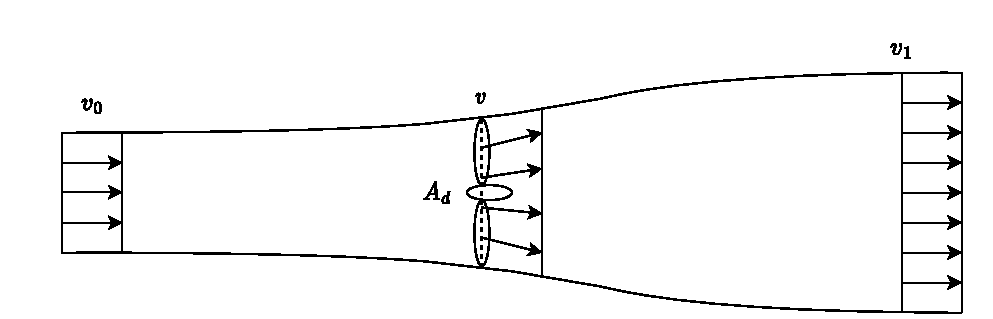
\includegraphics[width=0.8\linewidth]{Graphics/FlowThroughRotor.pdf}
	\caption{Illustration of how the wind in a control volume (CV) changes volume due to its reduction of speed}
	\label{fig:betz}
\end{figure}
The power of the \textit{free wind} $ v_0 $ can be expressed from the wind mass flow $ \dot{m} $ through a control volume:
\begin{equation} \label{eq:power}
	P = \dfrac{1}{2} \dot{m} v_0^2
\end{equation}
The flow of mass can be expressed from the air density $ \rho $, the cross sectional area $ A_d $ of the CV at the rotor and the free wind speed $ v_0 $ like so:
\begin{equation}\label{eq:mass_deriv}
	\dot{m} = \rho A_d v_0
\end{equation}
Combining \cref{eq:power} and \cref{eq:mass_deriv} yields:
\begin{equation}\label{eq:power2}
	P_{air} = \dfrac{1}{2} \rho A_d v_0^3
\end{equation}
A \textit{power coefficient} $ C_p $ represents the percentage of the available power that is extracted from the wind:
\begin{equation}\label{eq:Cp}
	C_p = \dfrac{P_T}{P_{air}}
\end{equation}
Such that the extracted power $ P_T $ is defined:
\begin{equation}\label{eq:power_w_Cp}
	P_{T} = \dfrac{1}{2} \rho A_d v_0^3 C_p
\end{equation}
$ C_p $ is dependent on the rotor blade pitch $ \theta $ and the tip speed ratio (TSR) $ \lambda $. In the partial load region the main goal is to reach a maximum $ C_p $ by adjusting $ \theta $ and  $ \lambda $ to their optimal values:
\begin{equation}\label{eq:cp_optimal}
	C_p^\star = C_p(\theta^\star, \lambda^\star)
\end{equation}
Where $ * $ denotes the optimal value of a parameter with regards to $ C_p $ at a given wind speed. This will be further explained in \cref{sec:theory_ctrl}. The TSR is the ratio between the speed of the tip of the WT blade $ (\Omega R) $ where $ R $ is the distance from the center of the rotor and the blade tip and the incoming free wind $v_0$:
\begin{equation}\label{eq:tipspeedratio}
	\lambda = \dfrac{\Omega R}{v_0}
\end{equation}

The achievable size of $ C_p^\star $ is a matter of the WT design. The \textit{Betz limit} is the highest, optimal $ C_p $ that can be theoretically achieved and can be calculated to be:
\begin{equation}\label{eq:betzlimit}
	C_{pbetz} = 0.5962
\end{equation}
%Most often $ C_p $ is also the measure of efficiency for a WT, but a more intuitive efficiency is  calculate measure efficiency from the Betz limit extractable power:
%\begin{equation}\label{eq:efficiency}
%	\eta = \dfrac{C_p}{C_{pbetz}}
%\end{equation}

%When the air travels over the WT blade the air travels slower on one side than the other as illustrated in \cref{fig:airfoil}. Due to mass conservation the air which moves slower on the underside of the blade expands, creating a higher pressure. Likewise the air moving faster on the upper upper side contracts creating in a lower pressure. Resultingly the blade moves upwards.
%\begin{figure}[ht]
%	\centering
%	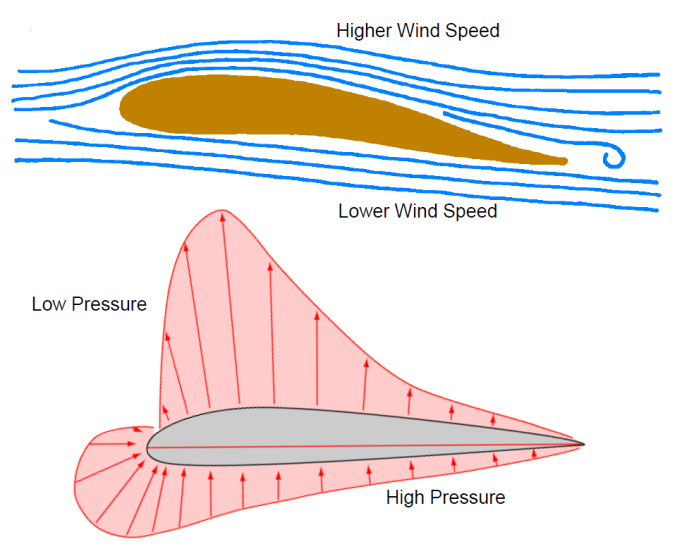
\includegraphics[width=0.5\linewidth]{Graphics/AirfoilAirflow.png}
%	\caption{Illustration of the wind speed difference between the two sides of a WT blade along with an illustration of the induced pressure difference. The result is a lifting force one the blade.}
%	\label{fig:airfoil}
%\end{figure}

Blade element momentum theory is often used to model the forces acting along WT blades. Blade element theory involves breaking a blade into small sections and determining the forces acting on each small section. In \cref{fig:blade_vel_triangles} a cross section of a WT blade can be seen. As also illustrated in \cref{fig:betz} the wind velocity that hits the rotor blades is lowered, indicated by the \textit{axial induction factor} $ a $. What is not observed in \cref{fig:betz} is that some of the energy of the wind also goes into driving an airstream around the back of the rotors in the opposite direction of the blade rotation, indicated by the \textit{tangential induction factor} $ a' $. This is known as \textit{swirl losses}. The induction factor's effect on the effective wind speed as seen by the rotor blade is observed in \cref{fig:blade_vel_triangle}. The $ \Omega r (1+a') $ term indicates that the effective wind speed parallel to the rotor plane is reduced by $ a' $ because $ a' < 1 $.
\begin{figure*}[ht]
	\centering
	\subfloat[Blade cross section]{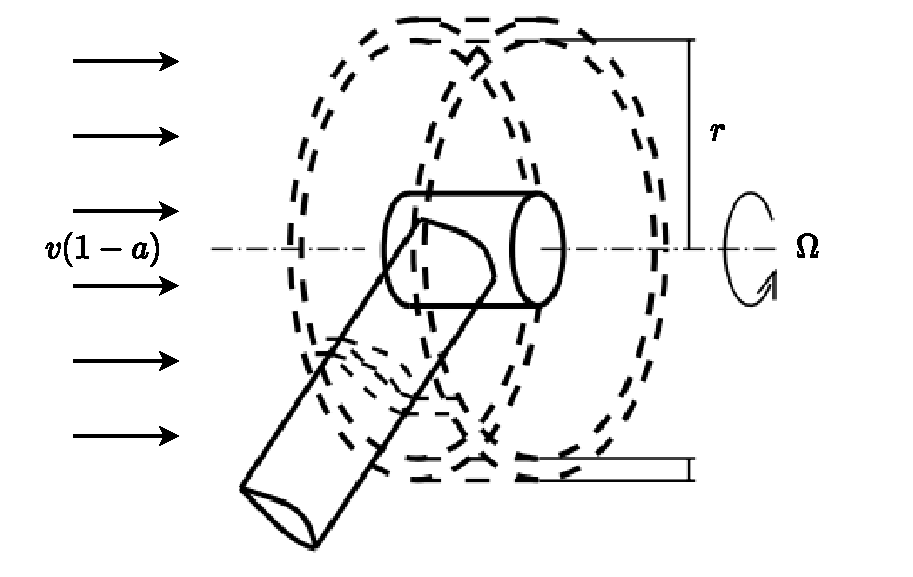
\includegraphics[width=.44\textwidth]{Graphics/RotorBladeElement.pdf}%
		\label{fig:blade_vel_triangles}}
	\hfil
	\subfloat[Velocity triangle]{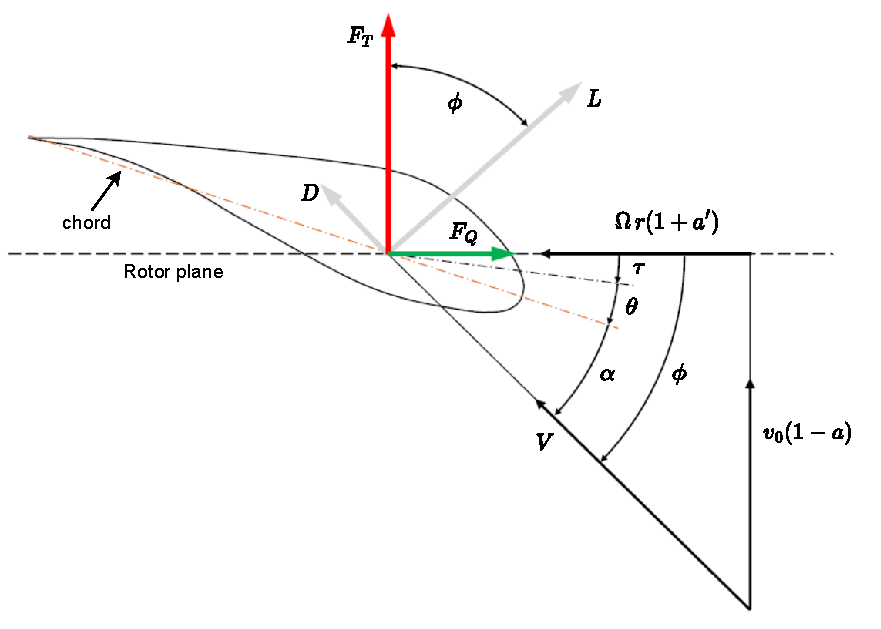
\includegraphics[width=.55\textwidth]{Graphics/BladeVelocityTriangle.pdf}%
		\label{fig:blade_vel_triangle}}
	\caption{Illustrations of a blade cross section and a velocity triangle on a blade section; \textbf{(a)} the blade cross section is made at some distance $ r $ from rotor center and rotates at a frequency $ \Omega $; \textbf{(b)} the velocity triangle acting on a cross section of a WT blade}
	\label{fig:blade_triangles}
\end{figure*}
The resulting air speed is V with an \textit{inflow angle} $ \phi $. $ F_L $ and $ F_D $ are the lift and drag forces on the blade element respectively. They are calculated from \cref{eq:lift} and \cref{eq:drag}. They include the \textit{chord length} $ c $ which is the length from the leading to the trailing edge of the blade.
\begin{align}
	F_L &= \dfrac{1}{2}\,  \rho \, V^2 c \, C_L \label{eq:lift}\\
	F_D &= \dfrac{1}{2} \, \rho \, V^2 c \, C_D \label{eq:drag}
\end{align}
The lift and drag coefficients $ C_L $ and $ C_D $ are usually extracted from table lookups which are typically found from simulations such as Xfoil
\todo{Hvad bruger Vestas til at finde $ C_L $ og $ C_D $?}. 
In a typical scenario $ C_L $ and $ C_D $ are found from the angle of attack $ \alpha $. The thrust and torque vectors $ F_T $ and $ F_Q $ are then calculated from the Pythagorean theorem as in \cref{eq:thrust} and \cref{eq:torque}
\begin{align}
	F_T &= L \, cos(\phi) + D \, sin(\phi) \label{eq:thrust} \\
	F_Q &= L \, sin(\phi) - D \, cos(\phi) \label{eq:torque}
\end{align}
The total thrust and torque of a blade can then be calculated by integrating the above over the length of the rotor blade \cite{Knudsen2013}.


\subsection{Wind turbine control} \label{sec:theory_ctrl}
This section includes a walk-through of the main functionality of WT control. The standard WT control scheme is explained with regards to different operation regions. Besides the main controller additional filters and controllers are implemented in the wind industry which mean to improve turbine performance, stability and safety. In this report only the main controller is included.

\medskip
In figure \cref{fig:controller_overview} a simplified illustration is seen of the Vestas turbine controller setup. It yields an overview of the main controllers that handle rotor/generator speed control and power control. The following section is focused on the responsibility of the partial load controller (PLC) and the full load controller (FLC). The depicted "Pitch Controller" and "Power Controller" of the diagram are black boxes from the point of view (POV) of this report. They are expected to follow their reference fast enough that it is irrelevant to model their dynamics.

PLC controllers can either be specified to output a torque or power reference and Vestas' controller outputs a power reference. Since the turbine at hand has a full scale converter all of the power delivery from the generator to the grid is handled by the electrical converter. The power reference $ P_{ref} $ output by the PLC sets the generator power $ P_g $ by means of the Power Controller.

\begin{figure}[ht]
	\centering
	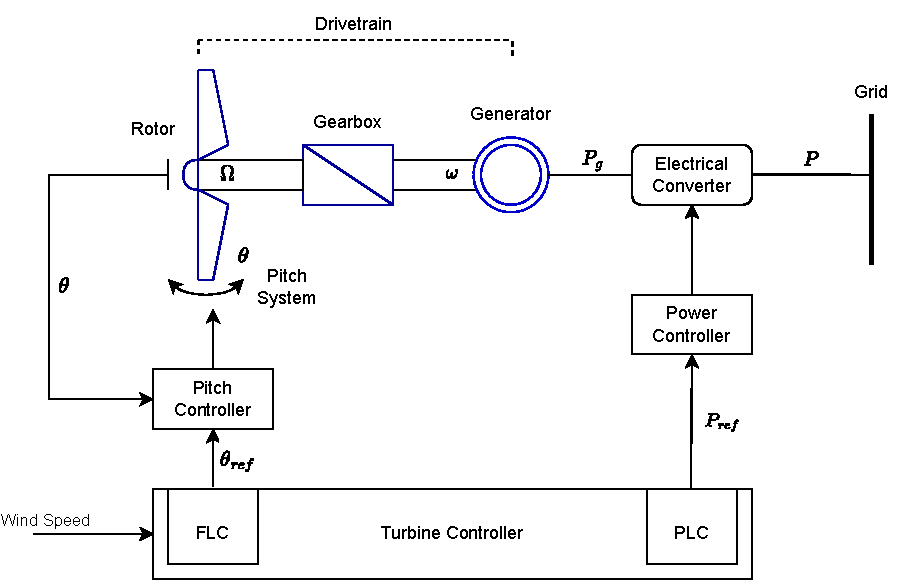
\includegraphics[width=0.7\linewidth]{Graphics/PLC_PI.pdf}
	\caption{An overview of the PLC/FLC controller setup. The turbine controller contains the FLC and PLC which gives a pitch reference to the pitch controller and a power reference to the power controller respectively.}
	\label{fig:controller_overview}
\end{figure}

\subsubsection{Control regions} \label{sec:theory_ctrl_regions}
Wind turbine control is split into two main stages of control: PLC and FLC. PLC is further split into three subregions. PLC is related to wind speeds between cut-in wind speed and rated wind speed. In all three PLC regions the generator power or torque reference is regulated with a PI controller based on a generator speed set-point to achieve the most optimal power output. The FLC region is related to the wind speed range from above rated to cut-out wind speed. In this region the pitch angle reference is regulated to track a constant rotor speed set-point and the generator power reference is constant at nominal power. Furthermore each of the four regions are associated with a specific wind speed range. A visualization of these operating regions can be found in figure \cref{fig:operating_regions}. The figure is simply illustrative and especially the width of the regions are out of proportion. 
\begin{figure}[ht]
	\centering
	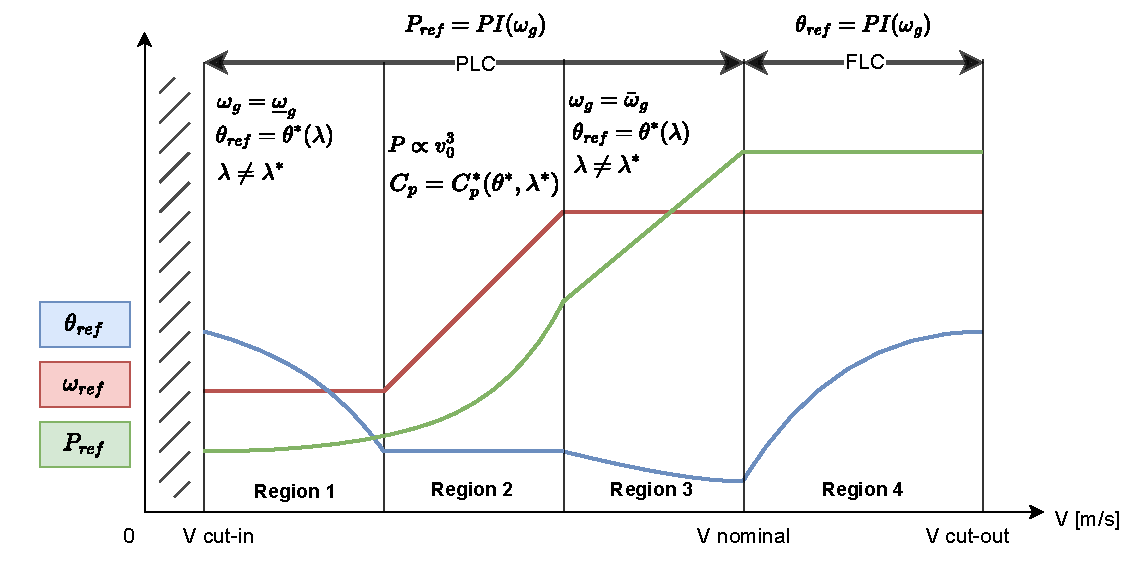
\includegraphics[width=0.9\linewidth]{Graphics/OperatingRegions.pdf}
	\caption{A visualisation of the wind turbine control operating regions. Specific wind speeds are purposefully not included since these are turbine specific. The figure is illustrative and not correctly scaled.}
	\label{fig:operating_regions}
\end{figure}
Below is a short description of the four regions focused on the parameters which are relevant to the control objective which is firstly maximisation of the turbine power output (PLC) and secondly limitation of the power output to nominal power (FLC). Below short descriptions are given to each of the WT operating regions as observed in \cref{fig:operating_regions}.
\begin{itemize}
	\item In \textbf{Region 1} the pitch angle reference is set to the optimal angle based on the tip speed ratio which in this region is \underline{not} optimal, meaning that $ C_p \neq C_p^* $ (where $ * $ denotes an optimal parameter value with regards to $ C_p $). The generator power is regulated to track the minimum rotor speed.
	\item In \textbf{Region 2} the pitch angle reference is set to the optimal angle. The tip speed ratio is optimal based on the generator speed which is controlled to the optimal value by means of the generator power. The rotor speed is proportional to the wind speed. The power output of the turbine is proportional to the third power of the wind speed which is intuitive given \cref{eq:power_w_Cp}.
	\item In \textbf{Region 3} like in region 1 the angle is set to the optimal angle based on the tip speed which is not optimal. The generator power is regulated to track the maximum rotor speed.
	\item In \textbf{Region 4} the pitch angle reference is no longer set at an optimal value. It is now set by the FLC PI controller which tracks a constant nominal rotor speed reference. In FLC the power output and rotor speed is ideally close to constant while the pitch angle changes to counteract changes in wind speed.
\end{itemize}



\subsubsection{Partial load control} \label{sec:theory_ctrl_plc}
PLC is active from cut-in wind speed to nominal wind speed. The highest priority of the \textbf{region 2} controller is to maximize $ C_p $ such that $ C_p(\theta, \lambda) = C_p^*(\theta^*, \lambda^*) $. Two actuators can potentially be utilized to control rotor speed to achieve this: Rotor pitch angle and generator torque. When observing a 3D plot of $ C_p(\theta, \lambda) $ such as the one in \cref{fig:cp_plot3d} it becomes apparent that maximisation of $ C_p $ will occur for specific values of $ \theta $ and $ \lambda $. In \cref{fig:cp_plot2d} the 3D plot is seen from above and thus only colours are indicators of the size of $ C_p $. Black lines are drawn on the plot which indicate a typical path from cut-in wind speed to cut-out wind speed starting in the top left corner where the tip speed ratio is very high due to the proportionally big difference between the minimum rotor speed and the low incoming wind speed and ending in the bottom right corner with the very high pitch angle. Furthermore the operating regions are drawn along the lines. It becomes obvious that all of regions 2 is centred at the $ C_p^*(\theta^*, \lambda^*) $ which is marked by a black dot in the middle of the darkest red region.
\begin{figure*}[ht]
	\centering
	
	\subfloat[$ C_p $ vs. $ \theta $ and $ \lambda $ (3D)]
	{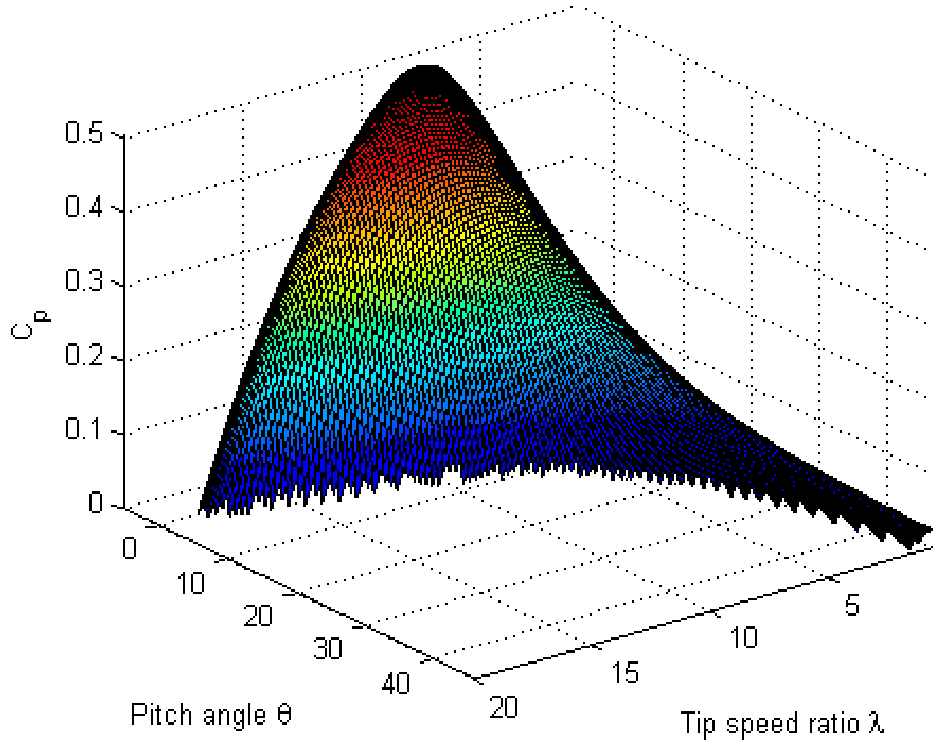
\includegraphics[width=.53\textwidth]{Graphics/Cp3dPlotV2.png}%
		\label{fig:cp_plot3d}}
	\hfil
	\subfloat[$ C_p $ vs. $ \theta $ and $ \lambda $ (2D)]
	{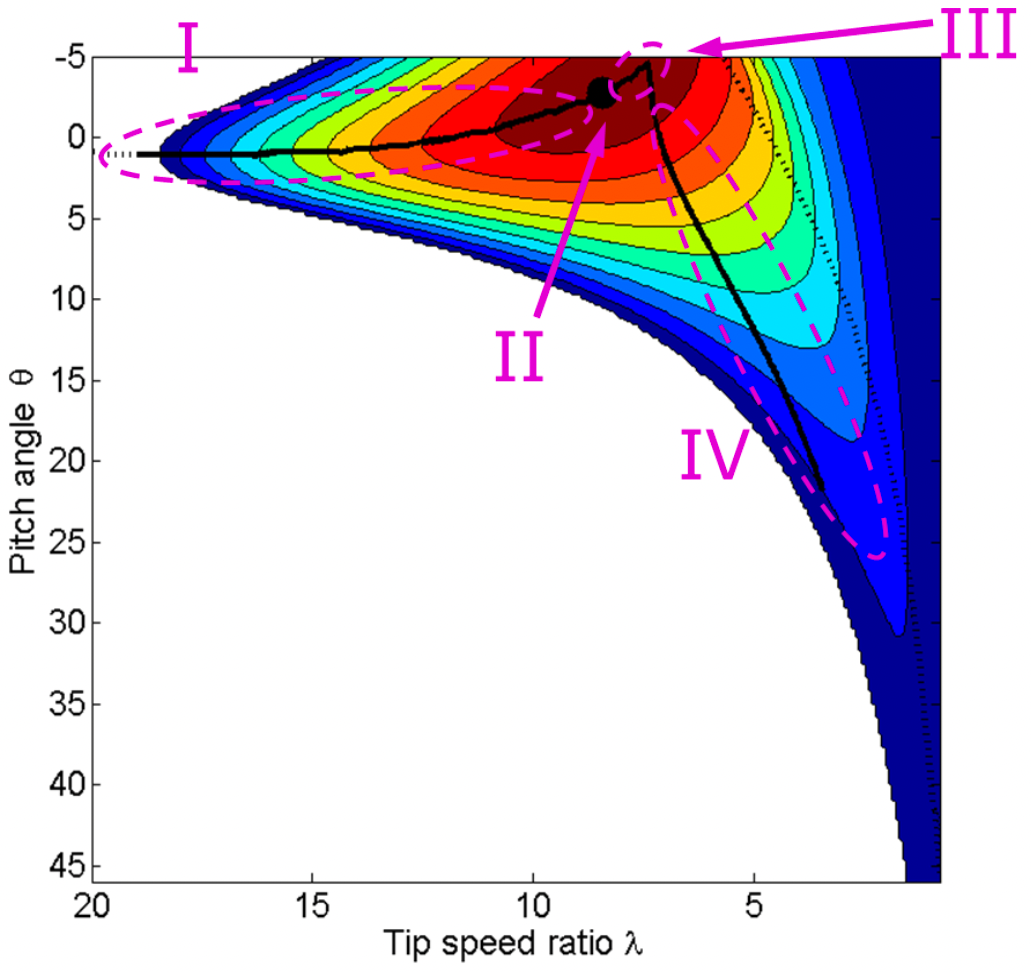
\includegraphics[width=.42\textwidth]{Graphics/Cp2dPlotRegions.png}%
		\label{fig:cp_plot2d}}
	
	\caption{Typical $ C_p $ plot drawn agains varying $ \theta $ and $ \lambda $; \textbf{(a)} 3D plot; \textbf{(b)} 2D plot where the operating regions are illustrated along the well. Figures are from internal LaC department material.}
	\label{fig:cp_plot}
\end{figure*}
$ \theta $ is determined from table lookups based on $ \lambda $ and thus cannot be utilized as an actuator to control the rotor speed such that $ \lambda(v_0, \Omega) = \lambda^*(v_0, \Omega^*) $ but the generator power can. Thus the primary concern is setting the generator power such that the rotor speed speed is optimal in relation to the wind speed. The rotor speed can in simplified form be described as in \cref{eq:rotor_speed_deriv}. The rotor speed increases when $ T_r > T_g $ and decreases when $ T_g > T_r $.
\begin{equation}\label{eq:rotor_speed_deriv}
	\dot{\Omega} = \dfrac{1}{J} \left( T_r(\theta, v_0) - T_g(P_g, \omega) \right)
\end{equation}
Here $ J $ is the total inertia of all parts connected to the drivetrain, $ T_r $ the rotor torque and $ T_g $ the generator torque referred to the rotor side of the drivetrain. From this equation it becomes apparent that if $ \theta $ is fixed at the optimal angle the generator torque is the only actuator available to control the rotor speed such that $ C_p = C_p^* $.

While there are numerous generator torque controllers in use in the wind industry the classical WT torque controller is defined as in \cref{eq:gen_torque_ctrl} where a generator torque is calculated based on the rotor speed.
\begin{equation}\label{eq:gen_torque_ctrl}
	T_g = K \Omega^2
\end{equation}
with the \textit{generator constant} being defined like so \cite{Pao2009}:
\begin{equation}\label{eq:gen_torque_const}
	K = \dfrac{1}{2} \rho \pi R^5 \dfrac{C_{p\_max}}{\lambda^{*3}}
\end{equation}
This causes the rotor speed to tend towards the optimal rotor speed. This is more readily visible when considering \cref{eq:omega_dot}. Consider when $ \frac{C_p}{\lambda^3} $ is greater than the optimal counterpart $ \frac{C_p^*}{\lambda^{*3}} $ then $ \dot{\omega} > 0 $ which will increase $ \omega $ until an increase in the $ \lambda^3 $ term will bring the two terms closer. $ \theta $ is fixed at $ \theta^* $ and therefore when $ \lambda^3 = \lambda^{*3} $ then $ C_p = C_p^* $ which is exactly the tracking goal.
\begin{equation}\label{eq:omega_dot}
	\dot{\Omega} = \dfrac{1}{2 J} \rho \pi R^5 \omega^2 \left( \dfrac{C_p}{\lambda^3} - \dfrac{C_p^*}{\lambda^{*3}} \right)
\end{equation}
\cref{eq:omega_dot} is derived by combining equations \cref{eq:power2}, \cref{eq:Cp}, \cref{eq:tipspeedratio}, \cref{eq:rotor_speed_deriv} and \cref{eq:gen_torque_ctrl} and \cref{eq:mech_torque}.
\begin{equation}\label{eq:mech_torque}
	T_r = \dfrac{P_T}{\Omega}
\end{equation}
\cref{eq:mech_torque} simply states the relationship between mechanical power $ P_T $, rotor speed $ \Omega $ and torque $ T_r $.

\medskip
Unlike the conventional torque controller, Vestas utilizes a PI controller structure for its PLC in all regions. The PI controller input is the generator speed error $ \omega_e $ multiplied with a gain scheduling contribution $ K_{gs}(\omega) $ which depends on the rotor speed:
\begin{equation}\label{eq:pi_plc_ctrl}
	P_{ref} = K_{gs}(\omega) \left(K_{plc,P} \, \omega_e + K_{plc,I} \int \omega_e\right)
\end{equation}
The generator speed reference in region 2 is calculated from the TSR formula in \cref{eq:tipspeedratio} with $ \lambda = \lambda^* $ like so:
\begin{equation}\label{eq:omega_ref_from_tsr}
	\omega_{ref} = v_0 \dfrac{\lambda^*}{R}
\end{equation} 
The mentioned gain scheduling component is present to account for the non-linearity of the system throughout the wind operating range.

In \textbf{region 1} achieving $ C_p = C_p^* $ is disregarded in favour of maintaining a minimum generator speed $ \underline{\omega} $. This is done to avoid the \textit{blade passing frequency} (3P) overlapping with the eigenfrequency of the system. The 3P frequency is the third multiple of the rotor frequency and this frequency is important with regards to resonance and fatigue loads. This concept is further explored in \cref{sec:theory_eigenfreq}. As such only $ \theta = \theta^* $.

\textbf{Region 3} is characterized by the generator speed reaching nominal speed $ \bar{\omega} $. Thus like in region 1 optimal $ C_p $ is disregarded to maintain the nominal generator speed. The output power has not reached nominal output power. Thus $ \theta = \theta^* $ and $ P_{ref} $ is regulated to achieve $ \omega = \bar{\omega} $. As the wind increases $ C_p $ decreases while $ P $ increases towards nominal power output. 

In both region 1 and 3 the PI controller is utilized. The generator speed reference is simply sat at $ \underline{\omega} $ in region 1 and $ \bar{\omega} $ in region 3.

The PI controller parameters $ K_{plc,P} $ and $ K_{plc,I} $ are tuned such that satisfactory performance and stability is achieved for a given turbine model. 

As the wind speed reaches the end of region 3 the generator power enters saturation and thus the WT control switches from PLC control to FLC control which is what the following section is concerned with.


\subsubsection{Full load control} \label{sec:theory_ctrl_flc}
FLC is active from nominal wind speed to cut-out wind speed. The generator speed reference is set to the constant nominal generator speed $ \bar{\omega} $. A PI controller tracks $ \bar{\omega} $ by regulating the collective pitch angle through $ \theta_{ref} $:
\begin{equation}\label{eq:pi_flc_ctrl}
	\theta_{ref} = K_{gs,dP/d\theta} \left(K_{flc,P} \, \omega_e + K_{flc,I} \int \omega_e\right)
\end{equation}
The PI controller output is multiplied with a gain scheduling term to compensate for the pitch-dependent sensitivity $ \frac{dP}{d\theta} $ which results from the non linear pitch authority \cite{Pao2009}. 

The power controller in FLC can be operated at either a constant power or constant torque set-point. Vestas' FLC controller operates with a constant power set-point with varying torque. This is favourable from a grid perspective because a steady power delivery is preferable but as a consequence a negative damping phenomena occurs with regard to the rotor speed. This negative damping phenomena should not be mistaken for the FOWT negative damping problem as they are two separate issues. The negative damping tendency becomes obvious when observing \cref{eq:rotor_speed_deriv} and considering the generator torque:
\begin{equation}\label{eq:gen_torque}
	T_g = \dfrac{P}{\omega}
\end{equation}
If for an example the generator speed decreases then the generator torque increases as a result of maintaining constant power. As a consequence the rotor speed deceleration increases even further. Consequently the FLC pitch controller must regulate the pitch more actively to compensate for the turbine's increased sensitivity to rotor speed changes.

The FLC PI controller parameters $ K_{flc,P} $ and $ K_{flc,I} $ are tuned such that satisfactory performance and stability is achieved for a given turbine model. 


\subsection{Eigenfrequencies and operating speeds} \label{sec:theory_eigenfreq}
When working with WT control it is relevant to understand the relationship between the eigenfrequencies of the WT tower and the forces that excite the turbine structure. The eigenfrequency of a system is the frequency at which that system oscillates after an initial disturbance has moved it from its equilibrium position.

A problem that both fixed-bottom and floating WTs have to deal with is frequency separation with regards to the natural frequencies of components and the periodic disturbances and exciting forces. Wind and waves will excite the tower at specific frequencies and it is important that such frequencies do not overlap with the turbine modes. Turbine towers are flexible will therefore oscillate. If a disturbance such as waves or the wind excite the WT at the same frequency as the natural frequency of the tower it will cause the tower to oscillate resulting in an increase in fatigue loads. Therefore towers are designed such that their first and second modes do not overlap with especially the 1P and 3P frequencies. 1P is the rotor rotational frequency and 3P known as the \textit{blade passing frequency} is the third multiple of 1P corresponding to the three blades of conventional horizontal WTs.
\begin{itemize}
	\item \textbf{1P} oscillations are typically activated by mass unbalance in the rotor blades.
	\item \textbf{3P} oscillations are typically activated by wind shear where the wind speed is higher at the rotor top than at the rotor bottom (individual blade pitching is utilized to dampen this effect).
\end{itemize}

A Campbell diagram such as the one seen in figure \cref{fig:campbell} is useful for visualizing the relationship between the allowed eigenfrequency of a component and the 1P and 3P frequencies. On the x-axis is the operating frequency of the turbine in revolutions per minute [rpm]. On the y-axis is the eigenfrequency in Hz. Lines are drawn for $ \pm 5 \% $ of both 1P and 3P. For any given turbine the box drawn between the 1P and 3P regions must not touch the lines drawn for the 1P and 3P regions. It becomes apparent why a clear operating region for the turbine rotor speed is defined. For a tower whose operating region is situated between 1P and 3P: If the lower boundary of the rotational speed is lowered the allowable eigenfrequency range decreases. At some point the operating region will have to cross the 1P lines which as explained will cause resonance and as a result increased fatigue loads \cite{Valentine2015}.
\begin{figure}[ht]
	\centering
	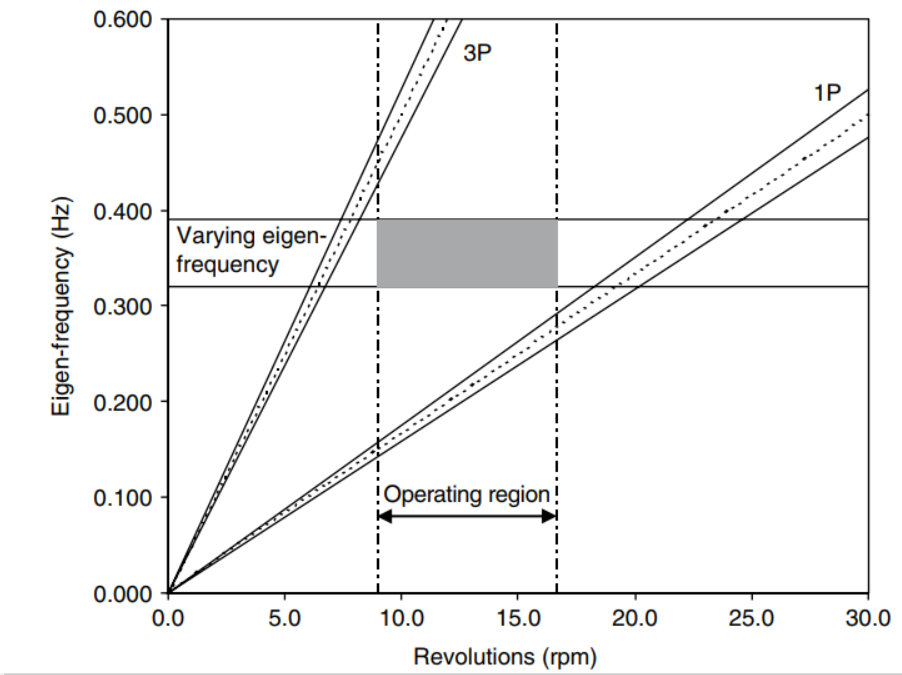
\includegraphics[width=0.5\linewidth]{Graphics/CampbellDiagram.PNG}
	\caption{The Campbell Diagram with the rotation frequency on the x-axis and the eigenfrequency on the y-axis. Figure from \cite{Valentine2015}}
	\label{fig:campbell}
\end{figure}
Modern WT towers with a \textit{soft-stiff} tower design are made such that their first eigenfrequency ends up between the 1P and 3P and the second eigenfrequency ends up above the 3P frequency. Some literature such as \cite{Dykes2018} denote tower designs as \textit{soft-soft}, \textit{soft-stiff} or \textit{stiff-stiff} depending on the position of the first tower eigenfrequency with regards to the 1P and 3P frequencies. As illustrated in the Campbell Diagram due to varying rotational frequency both 1P and 3P cover a range of frequencies. This is further illustrated in \cref{fig:1p_and3p} which furthermore highlights the possible eigenfrequency ranges of tower designs. In the diagram the natural frequency of FOWTs can be observed in frequencies way lower than 1P. The dotted line  just below the 3P frequency resembles the approximate location of the second tower mode. Its location close to 3P can cause unwanted oscillations.
\begin{figure}[ht]
	\centering
	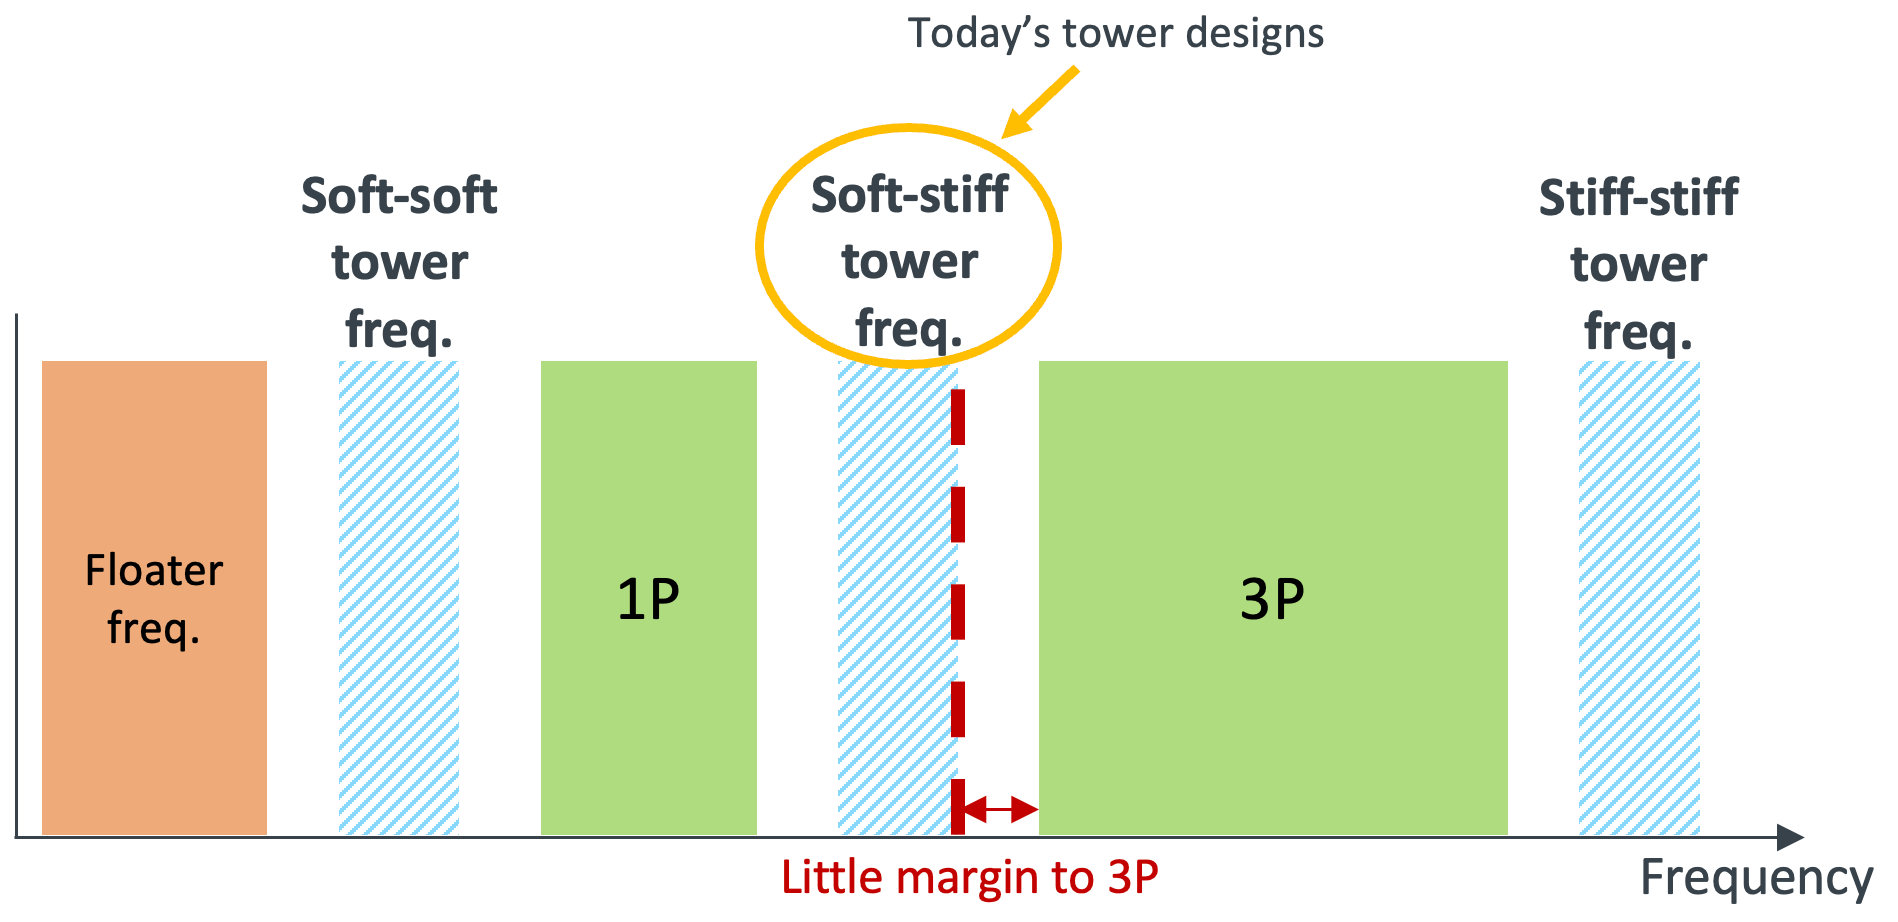
\includegraphics[width=0.7\linewidth]{Graphics/1Pand3PvsTwrStiff.PNG}
	\caption{Illustration of the frequency regions of the tower modes with different designs and for floaters as well as 1P and 3P. Figure is from internal LaC department material made by Thea Vanelli.}
	\label{fig:1p_and3p}
\end{figure}
In \cref{fig:eigen_and_1p3p} an illustration of the tower modes of both fixed-bottom and floating WTs is found. It is apparent that the first tower mode in a conventional fixed-bottom turbine is due to the flexion of the tower while in the floating structure it is due to the tilting of the whole turbine structure. Thus the conventional first tower mode of a fixed bottom turbine becomes the second mode of a floating turbine.
\begin{figure}[ht]
	\centering
	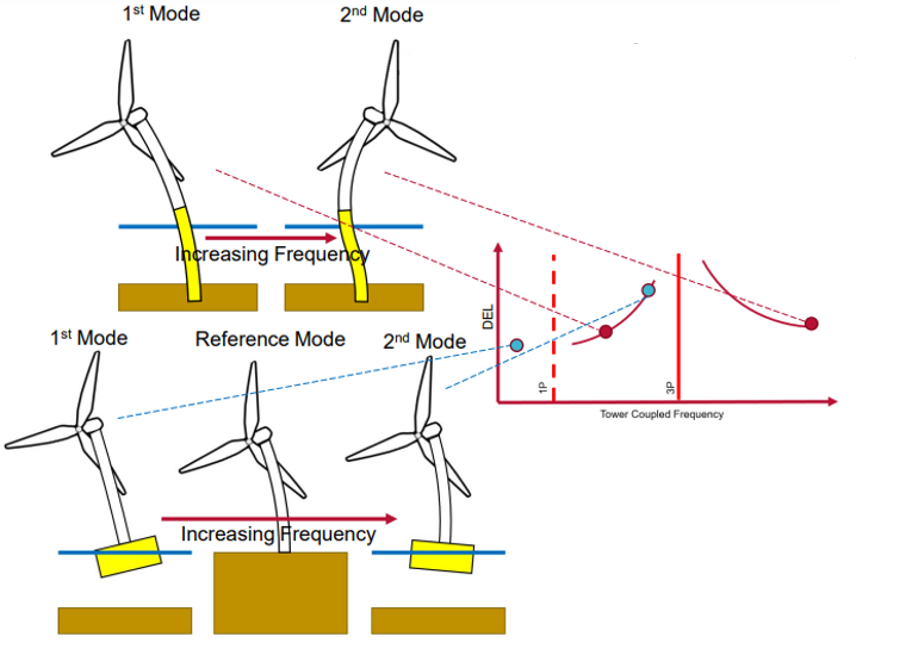
\includegraphics[width=0.7\linewidth]{Graphics/1P3PandEigenFloater.png}
	\caption{Illustration of the 1st and 2nd tower mode of both fixed-bottom and floater turbines. With floating structure the 1st mode is shiften down way past the 1P frequency. Figure is from internal LaC department material made by Thea Vanelli.}
	\label{fig:eigen_and_1p3p}
\end{figure}

\clearpage \newpage
\subsection{FOWT challenges and control} \label{sec:theory_fowt_challenges}
This section concerns the challenges that are prevalent in FOWT design and control. In the introduction of the FOWT in \cref{sec:intro_theFOWT} a specific issue; the negative dampening problem, was briefly described. This phenomena is further explored here and other relevant challenges are furthermore touched upon. Furthermore a few solutions to the negative dampening problem are briefly explained.

\medskip
To get a better understanding of the negative damping problem \cref{fig:thrust_vs_windspeed} is considered. It shows the relationship between wind speed and rotor thrust during operation where the turbine controller is actively regulating power in PLC and rotor pitch in FLC. The specific curve is from the IEA 15 MW reference wind turbine which is the subject of discussion in \cite{Vanelli2021}. The general shape of the curve is not turbine specific for modern turbines. The curve is a product of the relationship between pitch angle, wind speed and rotor speed which is regulated by the WT controller:
\begin{equation} \label{eq:aero_thrust}
	F_T(\theta, \Omega, v) = \dfrac{1}{2} \rho A_d v^2 C_T(\theta, \Omega, v)
\end{equation}
$ C_T $ is the thrust coefficient. In \cref{sec:theory_aero} the rotor thrust was defined for a blade from integrating over the thrust component of each blade element based on a combination of the lift and drag forces. When calculating the total stationary thrust it is convenient to use the pre-calculated thrust coefficient values $ C_T $ to determine the thrust \cite{Knudsen2013}. From \cref{eq:aero_thrust} the rotor thrust's dependency on $ v $ is obvious because of the $ v^2 $ term. The thrust's sensitivity to rotor speed and and pitch angle can only be inferred from the thrust coefficient's sensitivities to said variables. 
\begin{figure}[ht]
	\centering
	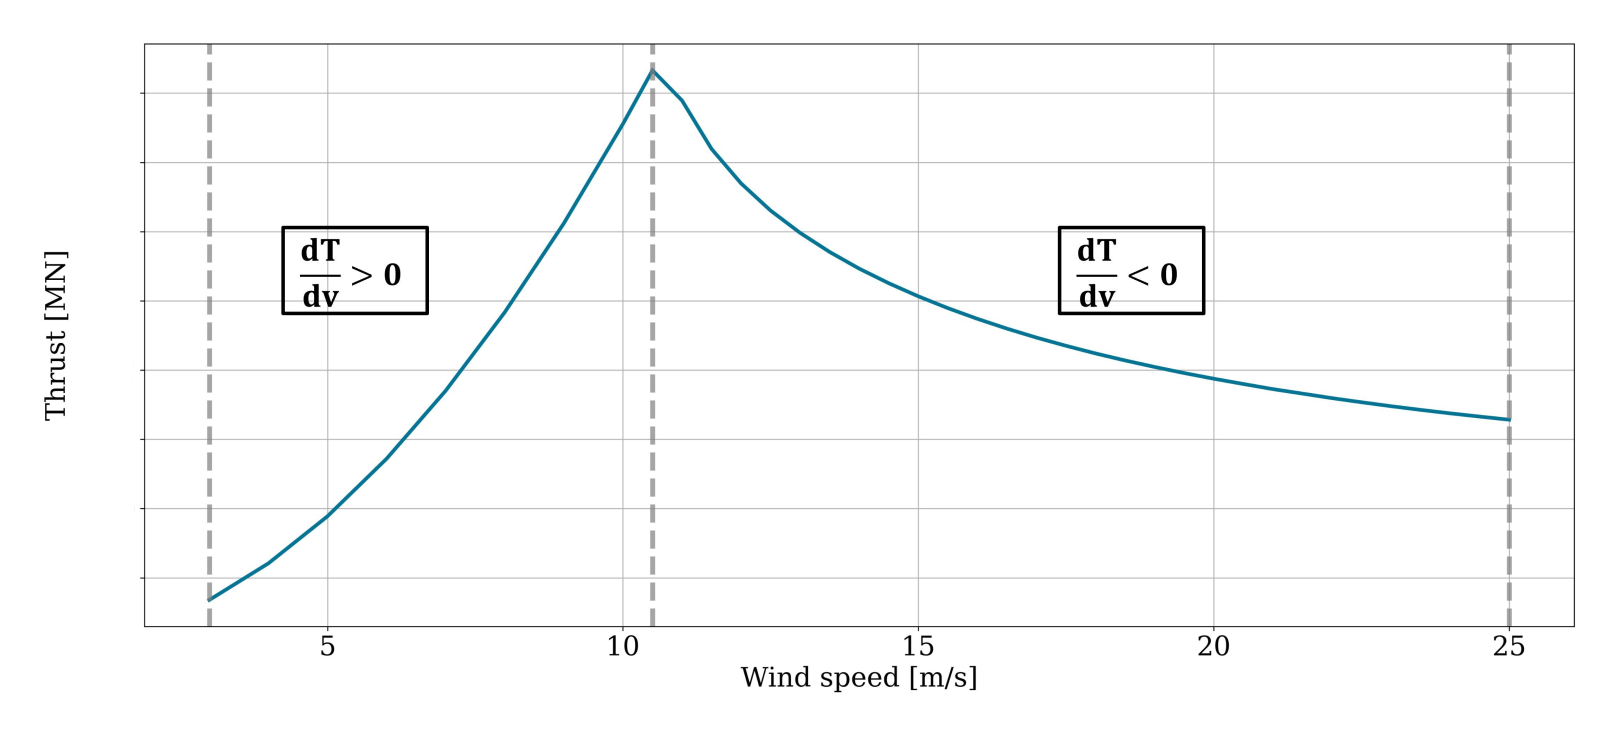
\includegraphics[width=0.85\linewidth]{Graphics/ThrustWindpeedCurve.PNG}
	\caption{Rotor thrust as a function of wind speed for the IEA 15 MW reference wind turbine. Figure from \cite{Vanelli2021}.}
	\label{fig:thrust_vs_windspeed}
\end{figure}
In \cref{fig:thrust_vs_windspeed} it is evident that rotor thrust increases until nominal after which the thrust decreases rapidly again. The increase in thrust before nominal is a product of the increased wind speed and the pitch angle which is either constant or decreasing in PLC as observed in \cref{fig:operating_regions}. An increase in wind speed always yields greater thrust and the FLC keeps the rotor speed constant. Thus the drop in thrust after nominal is due to the FLC increasing the pitch angle to limit the generator.

% In most of the operating range $ \dfrac{\partial C_T}{\partial \theta} < 0 $ something something.
The wind speed seen by the rotor is a function of the free wind speed and the fore-aft motion: $ v = v_0 - v_y $. $ v_y $ is the velocity of the nacelle in the surge direction and a \textit{backwards motion} refers to a positive movement in this direction. Consider a given wind speed in FLC: If the turbine moves backwards, $ v_y $ increases, resulting in a lowered wind speed $ v $ seen by the rotor. When observing \cref{fig:thrust_vs_windspeed} it is obvious that the thrust increases for lower wind speed. This causes the turbine to move backwards even faster. In the other scenario when the turbine moves forward the wind speed seen by the rotor increases, resulting in an even lower thrust, causing the turbine to move forward with even less resistance. If not properly addressed the result of this behaviour is instability or standing oscillations around the turbine pitching axes. The test journal in the appendix in \cref{app:tj_02} documented the oscillations resulting from normal FLC operation without a fore-aft motion mitigation strategy. At average wind speeds of 14 m/s and 16 m/s the tower top position oscillates between xx and xx m with a period of xx seconds. \todo[inline]{Udfyld disse tal fra }

This phenomena is present in both fixed bottom and floating WTs but the problem is greatly exacerbated for FOWTs due to their extra degrees of freedom. For fixed bottom turbines a solution is to detune the controller bandwidth below the system's first natural frequency. The resulting control performance is usually satisfactory. Vestas' solution is their fore-aft tower damper (FATD) controller addition. In the simplest case the FATD takes the nacelle's horizontal acceleration in the surge direction as input and outputs a collective pitch angle contribution $ \theta_{FATD} $ which is added to the pitch reference:
\begin{equation}\label{eq:fatd}
	\theta_{ref} = \theta_{flc} + \theta_{fatd}
\end{equation}
If the same fore-aft motion mitigation strategies used for fixed bottom WTs are used for floating turbines severe instability issues can ensue \cite{Larsen2007}. Therefore another strategy or tuning must be adopted to handle the negative damping problem on floating turbines. Several solutions are known with the simplest being to detune the FLC to below the first natural frequency of the FOWT. While it solves the problem it is a poor solution yielding big rotor speed variations as a result of the very slow rotor speed controller. Other common methods include feeding back the tower top velocity or acceleration through filters to a PI controller which outputs a pitch reference contribution \cite{Grant2022}. Vestas adopts a variation of this method which coincidentally is simply a heavily detuned version of their FATD. As it stands, tuning of the FATD is mostly trail and error and does not rely on a linear model. \todo[inline]{Er det rigtigt at FATDen ikke er baseret på en model? Jeg forsøger blot at komme lidt af en forklaring på hvorfor mit projekt er relevant :)}

Furthermore as mentioned in \cref{sec:theory_ctrl_flc} constant power control results in a negative damping term with regards to the rotor speed. This plays an important role for stability since this strategy can result in over-speeding of the rotor in FOWTs. While the constant torque strategy seems to limit the rotor speed variation the improvement comes at the expense of some generator overloading due to the power increasing with rotor speed \cite{Jonkman2010}. As mentioned Vestas utilizes constant power tracking and thus this strategy is assumed in this project.